\section{Reflectie Lesdemo}
\label{sec:lesdemo}
Voor de lesdemo heb ik niet een bestaande les gepakt omdat dat niet zou aansluiten bij de voorkennis van de medestudenten in de Didactiekcursus. De les die ik gemaakt had was een korte introductie op een aantal begrippen in het programmeren met opdrachten die zelf uitgevoerd konden worden op ieders laptop. Zelf had ik het idee dat ik veel aan het woord was een kwaal die mij vaker overkomt. En dat ik soms wat te veel gas geef in de les. Ik wil graag dat iedereen erbij is. Daarbij geef ik dan heel veel energie met vragen als: \textit{"Is iedereen er nog bij? Kan ik verder"}, etc. Naar mijn idee komt dat nogal onrustig en opzweperig over. Bovendien houd ik dat ook niet lang vol. Een collega van mij verwoorde het zo:
\begin{quotation}
  \textit{"Ik zie dan Fritz de bandleider, dat mag echt wel rustiger. Het is geen concert."}
\end{quotation}
In de feedback van mijn medestudenten waren de overtonen positief: \textit{heel relaxed, op je gemak, leuk om mee te doen, goed gebruik van je stem, natuurlijk overwicht, goed gebruik van complimenten, enthousiast}. De tips zaten wat meer op de context en protocol: \textit{waar doen we dit voor, de transfer is niet helder, het mist wat structuur (wat, waarom en hoe), context ontbreekt.}
Kort gezegd miste de les wat omlijsting. Dit is een bekende valkuil van mij. Dit heeft ook bijgedragen aan het vormen van het leerdoel voor het onderdeel \textit{Activerende didactiek}. Voor de lessen neem ik mee dat ik wat meer ondertiteling wil geven aan het proces. Als ik bijvoorbeeld de studenten aan de slag laat met elkaars werk nakijken, geef ik daarbij aan dat ik dat bewust doe omdat ze er minder van zouden leren als ik het voordoe, dan wanneer ze er met elkaar over bakkeleien.
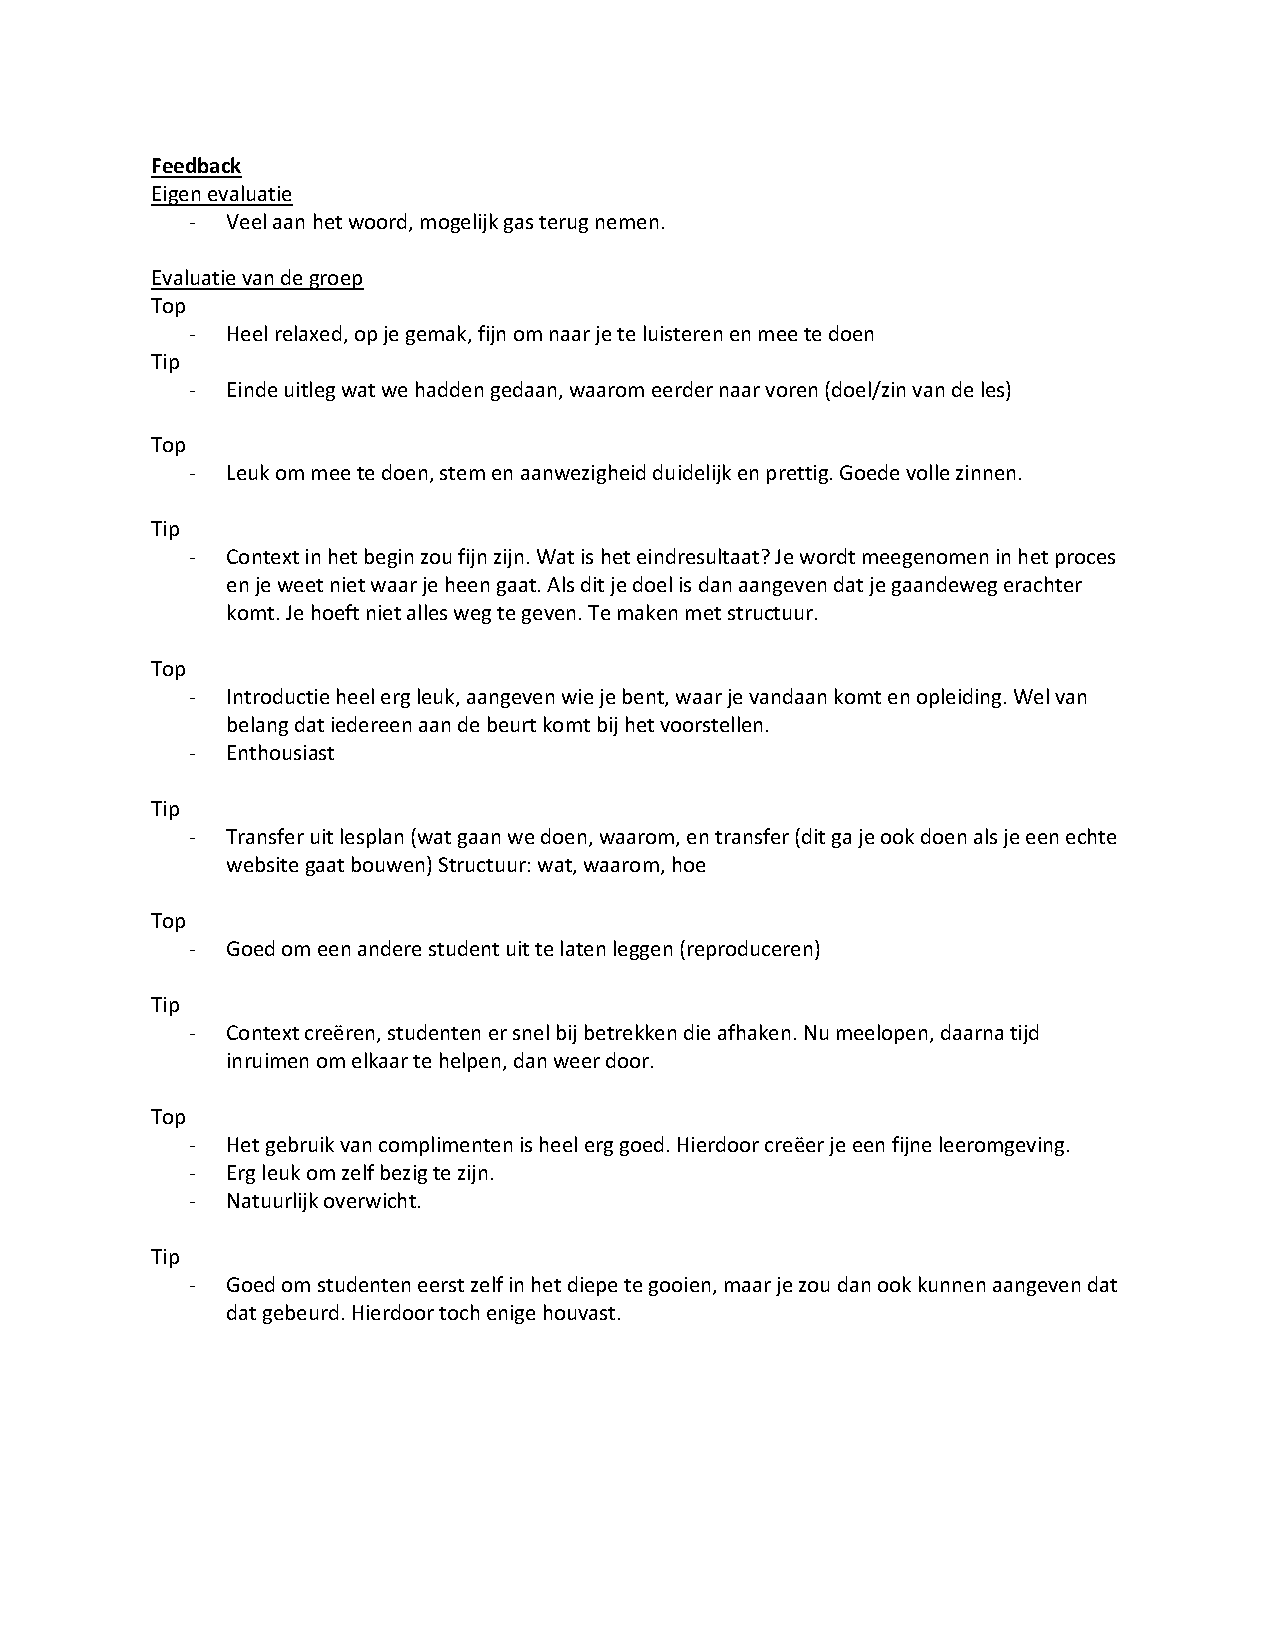
\includepdf[pages=-]{FeedbacklesdemoFritz22-5.pdf}
